% =====================================================================
%  WCCM 2026 / ECCOMAS — MS090E (Machine Learning for Computational
%  Mechanics Across Scales V), 22 July 2026, slot 4/6.
%  Defect estimation in perforated CFRP interstage structures (FEA + GNN).
%  Build: latexmk -pdf wccm_beamer.tex   (needs biber; references_gnn.bib)
% =====================================================================
\documentclass[aspectratio=169,10pt]{beamer}

\usetheme{metropolis}
\usecolortheme{default}

% ---- Times-family fonts (academic look) ----
\usefonttheme{professionalfonts}
\usepackage[T1]{fontenc}
\usepackage[utf8]{inputenc}
\usepackage{newtxtext,newtxmath}

\usepackage{booktabs}
\usepackage{amsmath,amssymb}
\usepackage{graphicx}
\usepackage{xcolor}
\usepackage{tikz}
\usetikzlibrary{positioning,arrows.meta}
\usepackage{array}

% ---- bibliography ----
\usepackage[style=numeric-comp,sorting=none,backend=biber,maxnames=2,giveninits=true]{biblatex}
\addbibresource{references_gnn.bib}
% citation の見た目調整: インライン [n] は小さめ＆LUHブルーで控えめに、一覧は scriptsize
\renewcommand*{\bibfont}{\scriptsize}
\AtEveryCite{\scriptsize\color{luhblue}}

\definecolor{luhblue}{RGB}{21,101,192}
\definecolor{luhdark}{RGB}{30,30,30}
\definecolor{alertred}{RGB}{198,40,40}
\definecolor{okgreen}{RGB}{27,94,32}

\setbeamercolor{frametitle}{bg=luhblue, fg=white}
\setbeamercolor{progress bar}{fg=luhblue}
\setbeamercolor{alerted text}{fg=alertred}
\setbeamercolor{example text}{fg=okgreen}
\metroset{progressbar=frametitle, block=fill}

\graphicspath{{figures/}{figures_paper/}{../results/}{../figures/}}

\newcommand{\best}[1]{{\color{okgreen}\textbf{#1}}}
\newcommand{\bad}[1]{{\color{alertred}#1}}

\title{Development of a Defect Estimation Method for CFRP Interstage
Structures with Holes using Finite Element Analysis and Graph Neural Networks}
\author[K.\ Nishioka et al.]{\underline{Keisuke Nishioka}\inst{1} \and Yuta Kojima\inst{2}
\and Toshiya Saito\inst{3} \and Masahito Washiya\inst{3}
\and Kosuke Kawakami\inst{3} \and Mayu Muramatsu\inst{4}}
\institute{\inst{1}Keio University, Sci.\ for Open \& Environ.\ Systems \quad
\inst{2}Nagoya University \\ \inst{3}JAXA, R\&D Directorate \quad
\inst{4}Keio University, Mech.\ Engineering}
\date{17th WCCM / ECCOMAS 2026, Munich \quad MS090E \quad (draft \today)}

% =====================================================================
\begin{document}

{\setbeamertemplate{footline}{}\maketitle}
\note{Session MS090E ``ML for Computational Mechanics Across Scales V'', 22 Jul 17:00,
slot 4/6. Only talk on a real engineering structure + NDT data pipeline + industrial
application; the others are PDE-solver / structure-preserving methodology.}

% ---------------------------------------------------------------------
\begin{frame}{Motivation: defect localization in CFRP interstage structures}
\begin{columns}[T]
\begin{column}{0.55\textwidth}
  \vspace{0.3em}
  CFRP carries primary load in reusable space transportation
  (high strength-to-weight). \textbf{Interlaminar delamination} around
  bolt holes critically degrades integrity.

  \vspace{0.7em}
  \textbf{Infrared stress measurement} (NDT) gives a full-field surface map
  of the \emph{sum of principal stresses} (DSPSS)~\cite{dulieubarton1998development,pitarresi2003review};
  sub-surface defects are inferred from it.

  \vspace{0.7em}
  \begin{alertblock}{Task}
  Per-node classification into 19 classes — \emph{in-plane defect region}
  $\times$ \emph{insertion layer} — directly on the FEA surface mesh.
  \end{alertblock}
\end{column}
\begin{column}{0.45\textwidth}
  \centering
  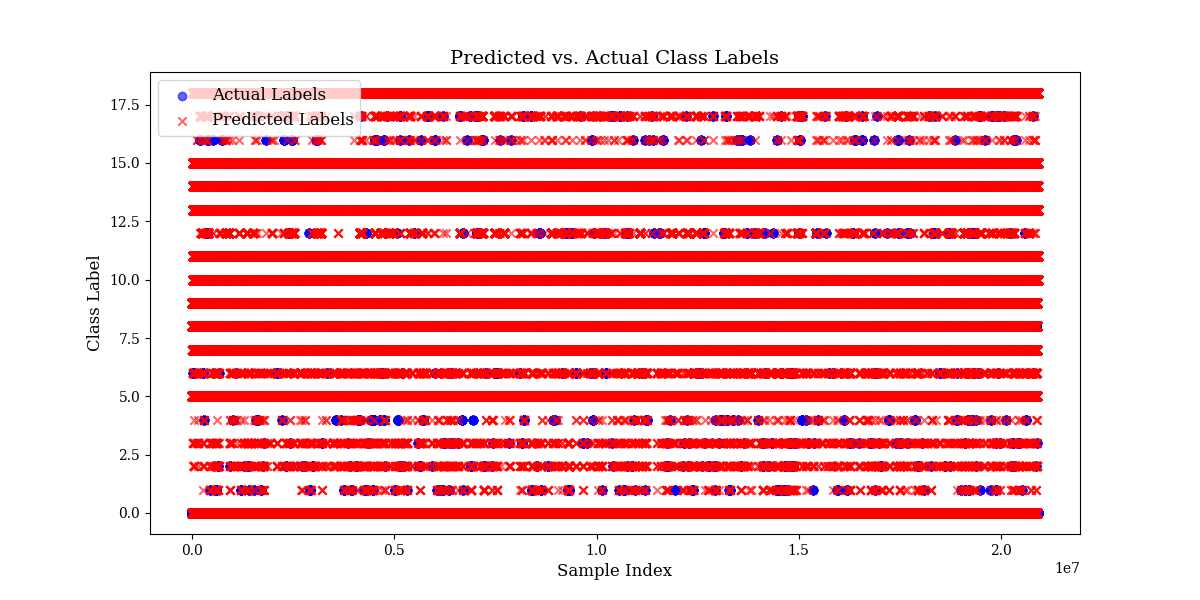
\includegraphics[width=\linewidth]{pred_vs_true.png}\\
  {\scriptsize Predicted vs.\ true node labels on the perforated specimen.}
\end{column}
\end{columns}
\end{frame}

% ---------------------------------------------------------------------
\begin{frame}{Prior work and scope of this talk}
\begin{itemize}
  \item \textbf{Prior framework} (Frontiers in Materials, 2025)~\cite{nishioka2025development}:
        a GAT-based GNN localizes defects in perforated CFRP from FEA-simulated DSPSS,
        with \emph{difference-normalized} inputs to suppress hole stress concentration.
  \item \textbf{This talk} extends it along two axes:
  \begin{enumerate}
    \item robustness under \emph{experimentally-motivated noise} + defect-free negatives;
    \item a controlled \textbf{architecture study} — from attention GNNs to
          \emph{mesh-physics} GNNs and four novel MeshGraphNet variants.
  \end{enumerate}
\end{itemize}
\vspace{0.4em}
\begin{block}{Data generation}
Synthetic FEA under tensile loading; interlaminar delamination modeled
explicitly by \textbf{Teflon inserts} between selected plies~\cite{nishioka2025development}.
\end{block}
\end{frame}

% ---------------------------------------------------------------------
\begin{frame}{Positioning within MS090E}
This minisymposium is dominated by \emph{PDE-solver / structure-preserving}
methodology. Our contribution is the only \textbf{real-structure NDT pipeline}:
\begin{itemize}
  \item vs.\ \textbf{thermodynamics-preserving GNNs} (Cueto et al.)~\cite{hernandez2022thermodynamics,hernandez2021structure}
        — they solve/constrain physics; we \emph{apply} GNNs to defect inference on real geometry.
  \item vs.\ \textbf{momentum-conserving physics-informed GNNs} (Sharma \& Fink)
        — dynamics/conservation; we address static thermoelastic DSPSS.
  \item vs.\ \textbf{Fourier-embedded PINN $\times$ DIC} (Liu \& Yi)~\cite{tancik2020fourier}
        — full-field experimental measurement; shared sim-to-real motivation.
\end{itemize}
\vspace{0.3em}
\begin{alertblock}{Three differentiators}
(1) real engineering structure \& NDT pipeline; \;
(2) extreme class imbalance (defects $<3\%$); \;
(3) baseline-free \& OOD generalization to unseen defect sizes.
\end{alertblock}
\end{frame}

% ---------------------------------------------------------------------
\begin{frame}{Data \& graph representation}
\begin{columns}[T]
\begin{column}{0.5\textwidth}
\textbf{One specimen $\rightarrow$ one graph}
\begin{itemize}
  \item $13{,}942$ nodes (two stacked plies around the hole)
  \item Node features: $[x,y,z,\text{DSPSS}]$
  \item Edges: FEA mesh connectivity, with coordinate-difference
        edge features $[dx,dy,dz,\lVert\cdot\rVert]$
  \item 19 classes (region $\times$ layer); class 0 = defect-free
\end{itemize}
\vspace{0.5em}
Input $=$ \emph{difference-normalized} DSPSS (damaged $-$ pristine)~\cite{nishioka2025development},
isolating the defect signal from hole stress concentration.
\end{column}
\begin{column}{0.5\textwidth}
\begin{exampleblock}{The imbalance trap}
Class-0 prior $\approx 0.998$. Predicting ``defect-free'' everywhere gives
$99.8\%$ accuracy yet \bad{macro-F1 $\approx 0$}.
\end{exampleblock}
\vspace{0.2em}
$\Rightarrow$ report \textbf{macro-F1}; engineer the training distribution,
not only the loss.
\vspace{0.3em}
\begin{center}
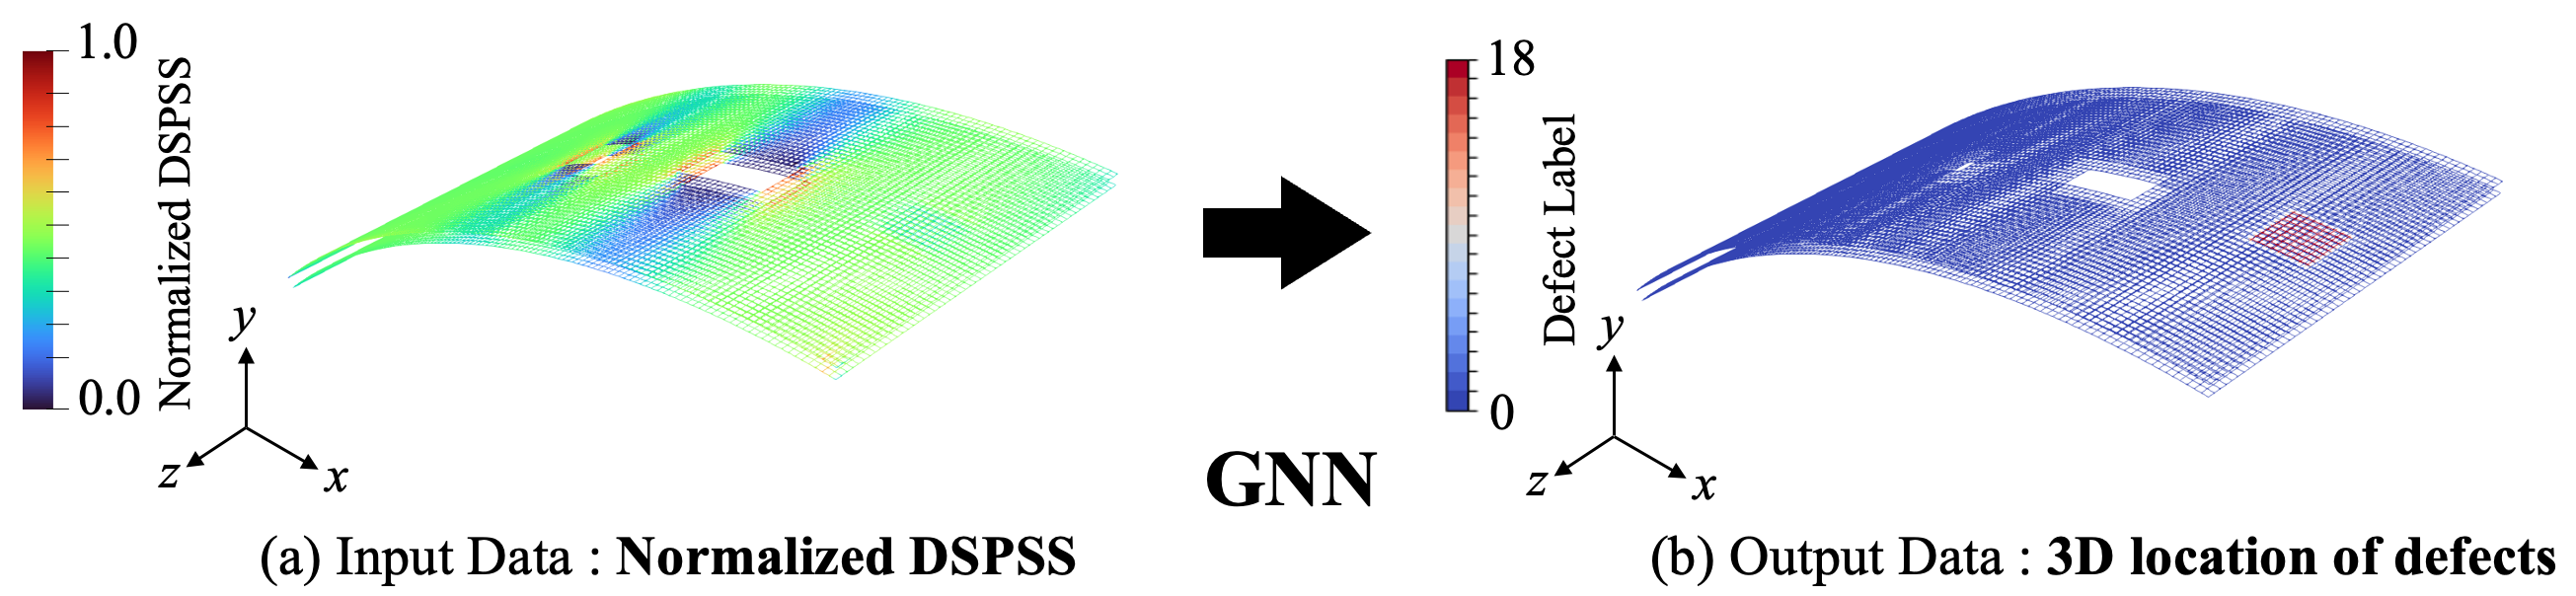
\includegraphics[width=0.92\linewidth]{gnn_graph_model.png}\\
{\scriptsize Surface mesh $\to$ node/edge graph.}
\end{center}
\end{column}
\end{columns}
\end{frame}

% ---------------------------------------------------------------------
\begin{frame}{Handling extreme class imbalance}
The recipe that makes learning possible:
\begin{enumerate}
  \item \textbf{Noise-augmented difference data} — robustness to acquisition noise~\cite{rong2020dropedge}.
  \item \textbf{Defect-free negatives (NDF)} — 5000 genuine class-0 graphs (train only).
  \item \textbf{Balanced sampling} 5000:5000 + \textbf{Focal loss}~\cite{lin2017focal}
        (cf.\ LDAM~\cite{cao2019learning}, logit adjustment~\cite{menon2020long},
        GraphSMOTE~\cite{zhao2021graphsmote}).
  \item Leakage control: group-purged val/test split by specimen.
\end{enumerate}
\vspace{0.5em}
\begin{alertblock}{Dominant factor}
With the recipe, a faithful reproduction reaches macro-F1 $\approx \textbf{0.70}$,
vs.\ $\le 0.08$ without it — the \emph{data distribution} dominates.
\end{alertblock}
\end{frame}

% ---------------------------------------------------------------------
\begin{frame}{Model zoo: from attention to mesh-physics GNNs}
\begin{tabular}{p{2.4cm} p{8.0cm}}
\toprule
Model & Mechanism \\
\midrule
\textbf{GAT}~\cite{velickovic2018graph} & attention over neighbours (Frontiers baseline). \\
\textbf{GATv2}~\cite{brody2022how} & \emph{dynamic} attention (strictly more expressive). \\
GraphSAGE & max-aggregation of neighbour features. \\
PNA & multiple aggregators + degree scalers. \\
\textbf{MeshGraphNet}~\cite{pfaff2021learning} & Encode-Process-Decode; node \emph{and} edge
  updates each step~\cite{sanchezgonzalez2020learning}. \\
\bottomrule
\end{tabular}
\vspace{0.4em}
All use coordinate-based geometric features (NDT-admissible). Equivariant
GNNs~\cite{satorras2021equivariant} considered as future structure-aware option.
\end{frame}

% ---------------------------------------------------------------------
\begin{frame}{Architecture sweep under the balanced recipe}
\centering
Identical recipe, 120 epochs, balanced 5000:5000, group-purged eval.
\vspace{0.4em}

\begin{columns}[T]
\begin{column}{0.56\textwidth}
\small
\begin{tabular}{lcl}
\toprule
Architecture & macro-F1 & note \\
\midrule
\best{MeshGraphNet}~\cite{pfaff2021learning} & \best{0.764} & Encode-Process-Decode \\
GATv2~\cite{brody2022how}             & 0.694 & dynamic attention \\
GAT~\cite{velickovic2018graph}        & 0.674 & Frontiers baseline \\
GraphSAGE                             & 0.663 & max-aggregation \\
PNA                                   & 0.613 & multi-aggregator \\
\bottomrule
\end{tabular}
\end{column}
\begin{column}{0.44\textwidth}
\centering
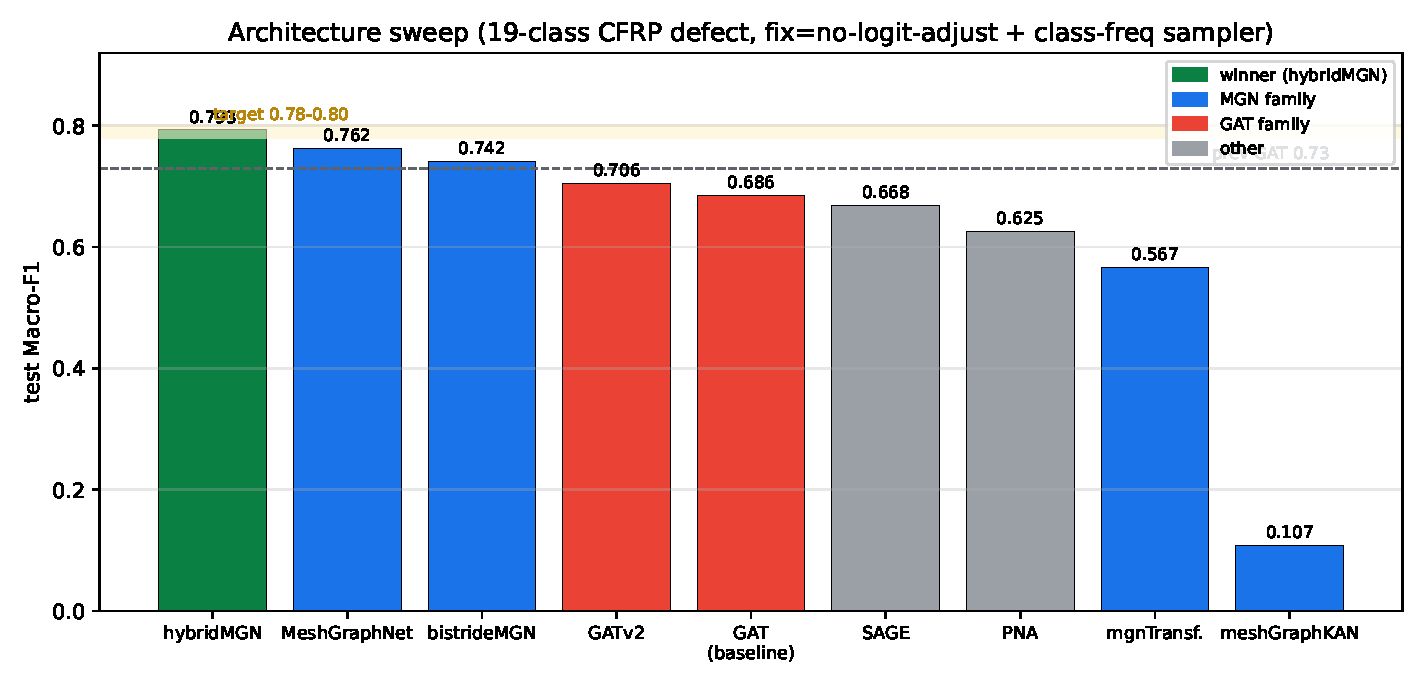
\includegraphics[width=\linewidth]{arch_sweep.pdf}\\
{\scriptsize macro-F1 by architecture (balanced recipe).}
\end{column}
\end{columns}

\vspace{0.5em}
\begin{block}{Takeaway}
Under the balanced recipe, the \textbf{mesh-physics architecture} wins —
beating the legacy GAT recipe (0.70) and the published baseline (0.61).
\end{block}
\end{frame}

% ---------------------------------------------------------------------
\begin{frame}{Why MeshGraphNet fits the problem}
\begin{columns}[T]
\begin{column}{0.55\textwidth}
\textbf{Encode--Process--Decode}~\cite{pfaff2021learning,sanchezgonzalez2020learning}:
\begin{itemize}
  \item node \emph{and} edge embeddings updated at every message-passing step (residual);
  \item edge feature $=$ coordinate difference $[dx,dy,dz,\text{dist}]$
        $\Rightarrow$ local geometry \& anisotropy;
  \item matches FEA-mesh stress-propagation structure better than attention-only GNNs.
\end{itemize}
\end{column}
\begin{column}{0.45\textwidth}
\centering
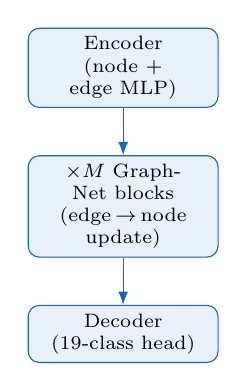
\begin{tikzpicture}[node distance=6mm, every node/.style={font=\scriptsize},
  box/.style={draw=luhblue, fill=luhblue!10, rounded corners, inner sep=3pt, text width=2.2cm, align=center}]
  \node[box] (e) {Encoder\\(node + edge MLP)};
  \node[box, below=of e] (p) {$\times M$ GraphNet blocks\\(edge\,$\to$\,node update)};
  \node[box, below=of p] (d) {Decoder\\(19-class head)};
  \draw[-{Latex}, luhblue] (e)--(p);
  \draw[-{Latex}, luhblue] (p)--(d);
\end{tikzpicture}
\end{column}
\end{columns}
\end{frame}

% ---------------------------------------------------------------------
\begin{frame}{Novelty: four MeshGraphNet variants for layered NDT}
\begin{tabular}{p{2.7cm} p{7.5cm}}
\toprule
Variant & Idea / why it could matter for CFRP \\
\midrule
\textbf{MeshGraphKAN} & Fourier-KAN node encoder — learnable spectral basis for the
  \emph{high-frequency stress-concentration} field (spectral-bias mitigation)~\cite{tancik2020fourier}. \\[2pt]
\textbf{Hybrid-MGN} & mesh edges $+$ \emph{front/back cross-layer ``world'' edges} —
  structurally separates the two plies. \\[2pt]
\textbf{BiStride-MGN} & per-graph global-context broadcast — multiscale, long-range
  stress propagation. \\[2pt]
\textbf{MGN-Transformer} & interleaved per-graph self-attention — global node interaction. \\
\bottomrule
\end{tabular}
\vspace{0.5em}
\begin{alertblock}{Hypothesis}
\textbf{MeshGraphKAN $\times$ stress concentration} and
\textbf{Hybrid-MGN $\times$ two-ply separation} are the two novel angles most
likely to cross macro-F1 $0.80$.
\end{alertblock}
\end{frame}

% ---------------------------------------------------------------------
\begin{frame}{Variant results}
\centering
\begin{tabular}{lcl}
\toprule
Variant & macro-F1 & vs.\ MeshGraphNet (0.761) \\
\midrule
\best{Hybrid-MGN}       & \best{0.792} & \textbf{+0.031} (new in-dist SOTA) \\
MeshGraphNet (baseline) & 0.761 & --- \\
BiStride-MGN     & 0.741 & $-0.020$ \\
MGN-Transformer  & 0.552 & $-0.209$ \\
MeshGraphKAN     & \texttt{TBD} & not yet run \\
\bottomrule
\end{tabular}
\vspace{0.4em}\\
{\scriptsize In-distribution eval (train on 2$\times$2/4$\times$4/8$\times$8 sizes, group-purged).}
\vspace{0.6em}

\begin{block}{Outcome (honest)}
Front/back cross-ply ``world'' edges (\textbf{Hybrid-MGN}) set a new
in-distribution SOTA at \textbf{0.792} --- best of all architectures, but
\emph{just short} of the 0.80 macro-F1 line. The cap is \textbf{adjacent-layer
confusion}, not architecture: exact 19-class accuracy already reaches
\textbf{0.85}.
\end{block}
\end{frame}

% ---------------------------------------------------------------------
\begin{frame}{Per-class performance \& confusion}
\begin{columns}[T]
\begin{column}{0.5\textwidth}
  \centering
  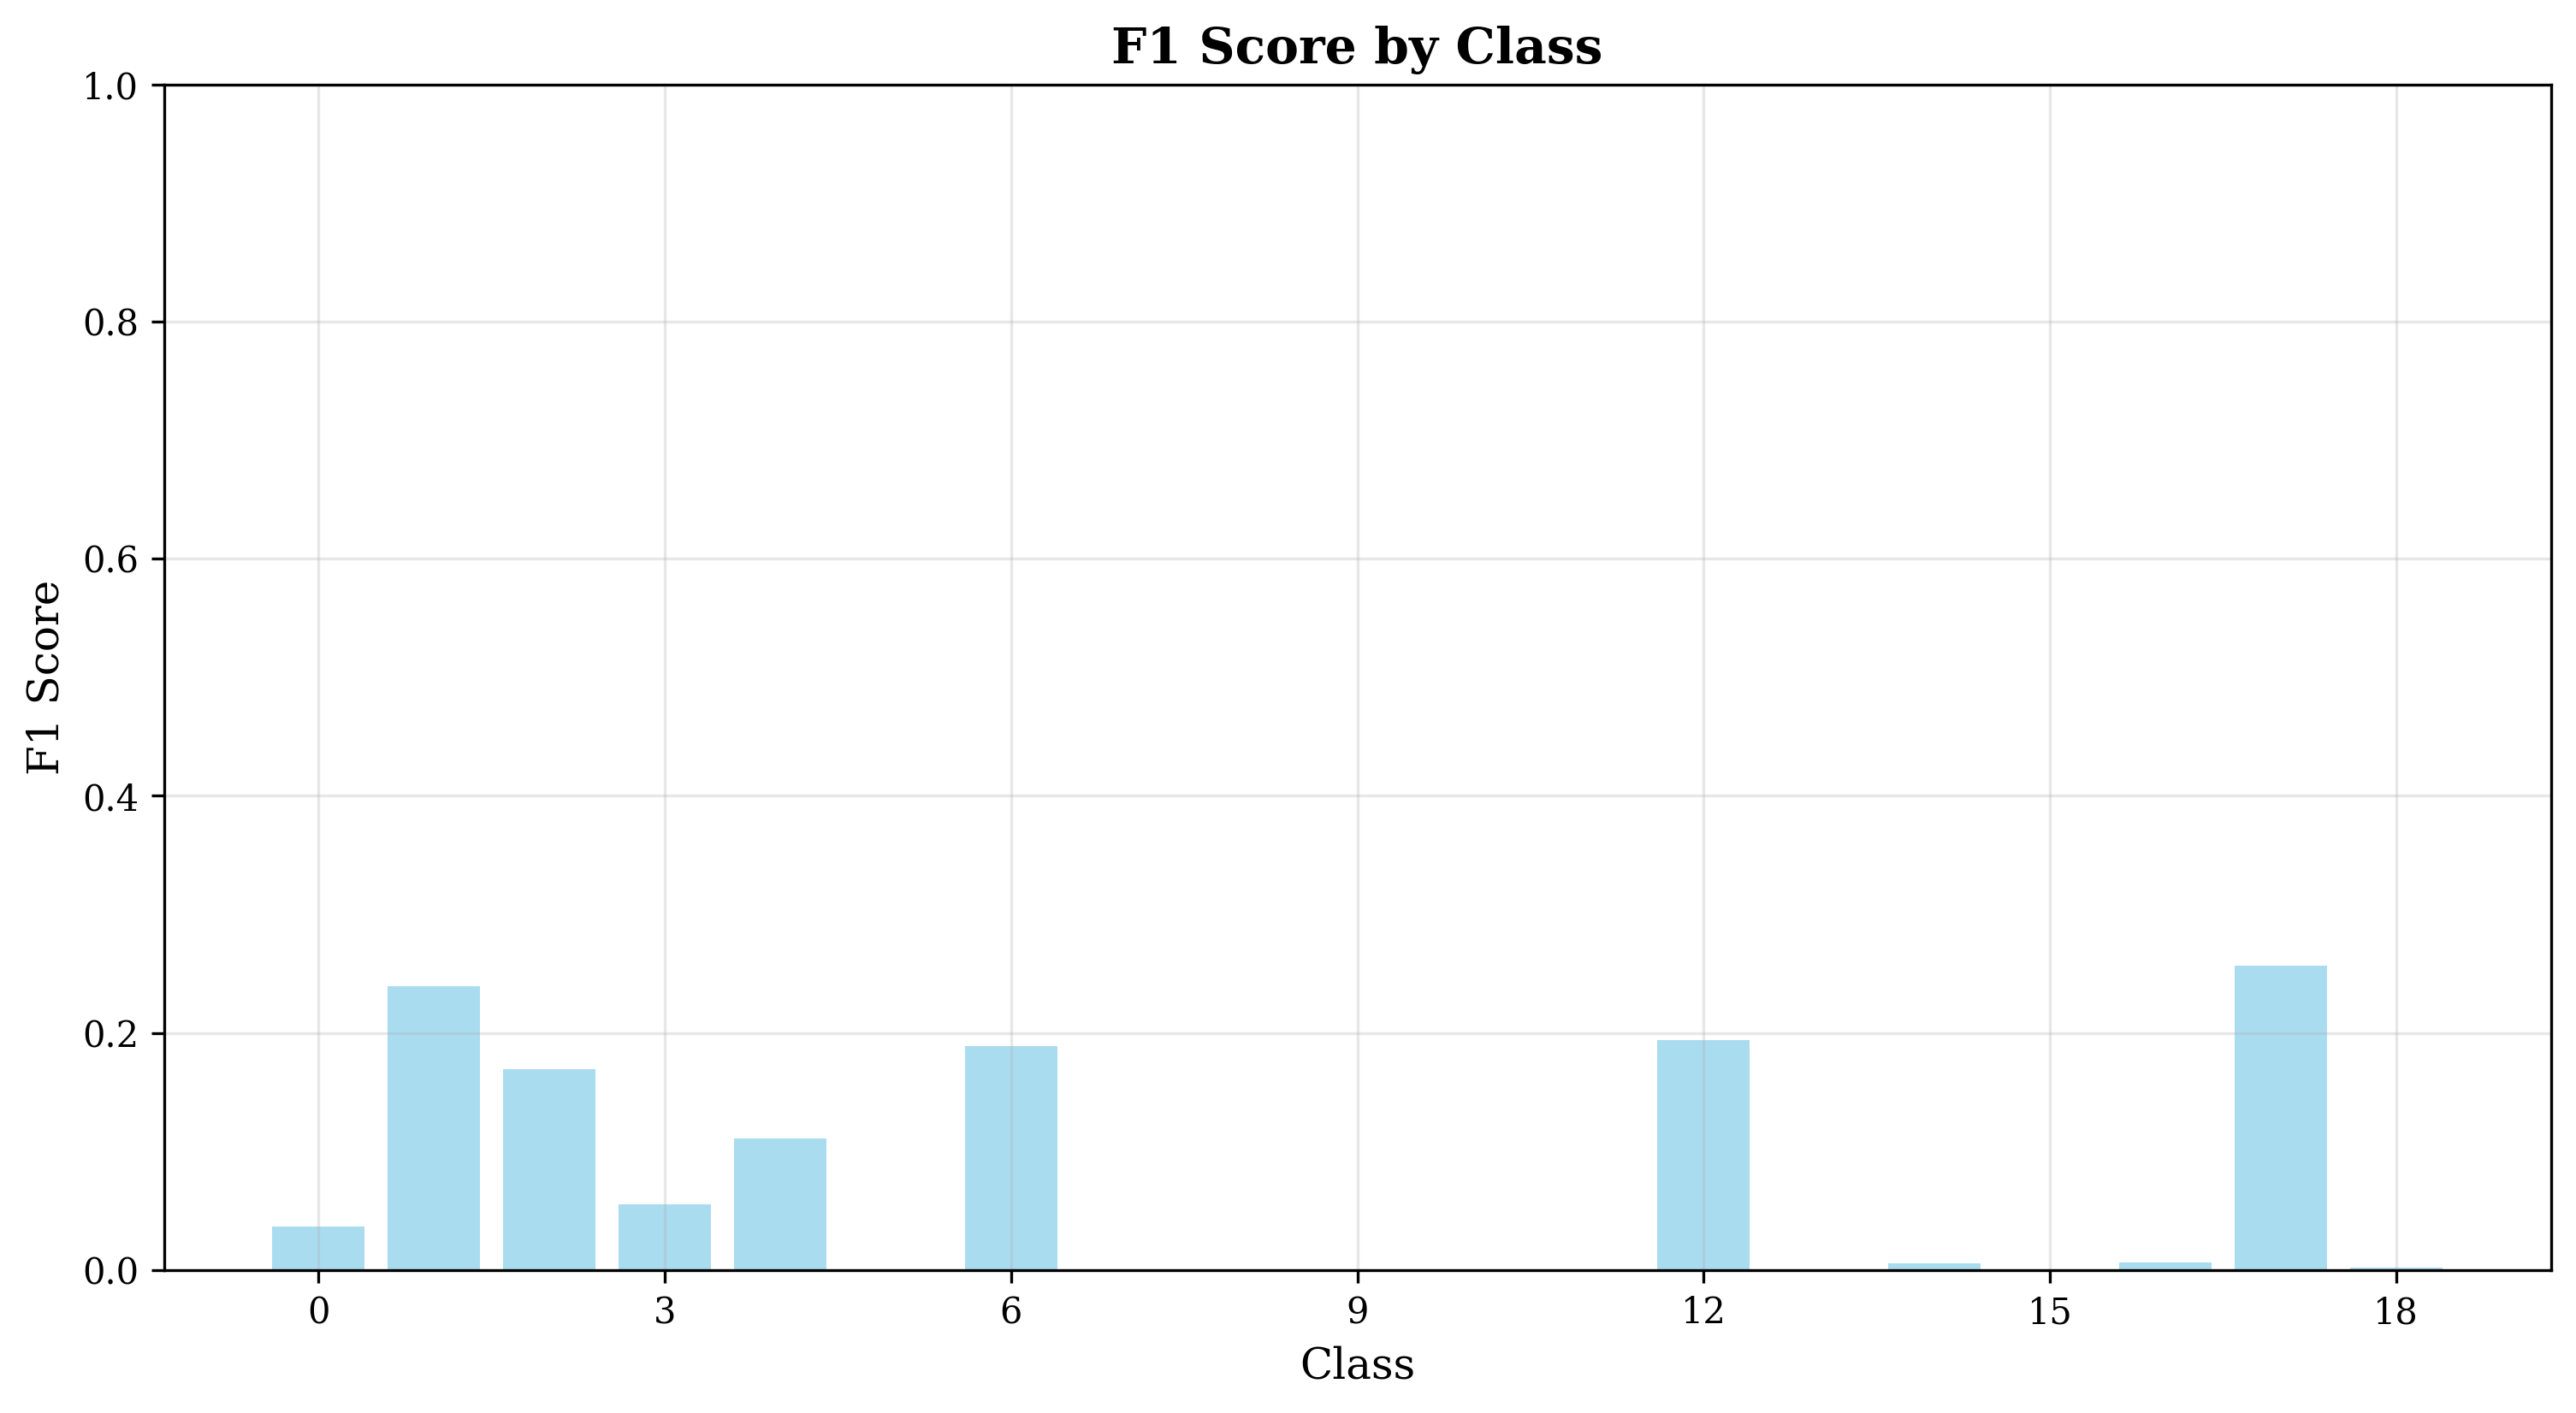
\includegraphics[width=\linewidth]{f1_per_class.png}\\
  {\scriptsize Per-class F1.}
\end{column}
\begin{column}{0.5\textwidth}
  \centering
  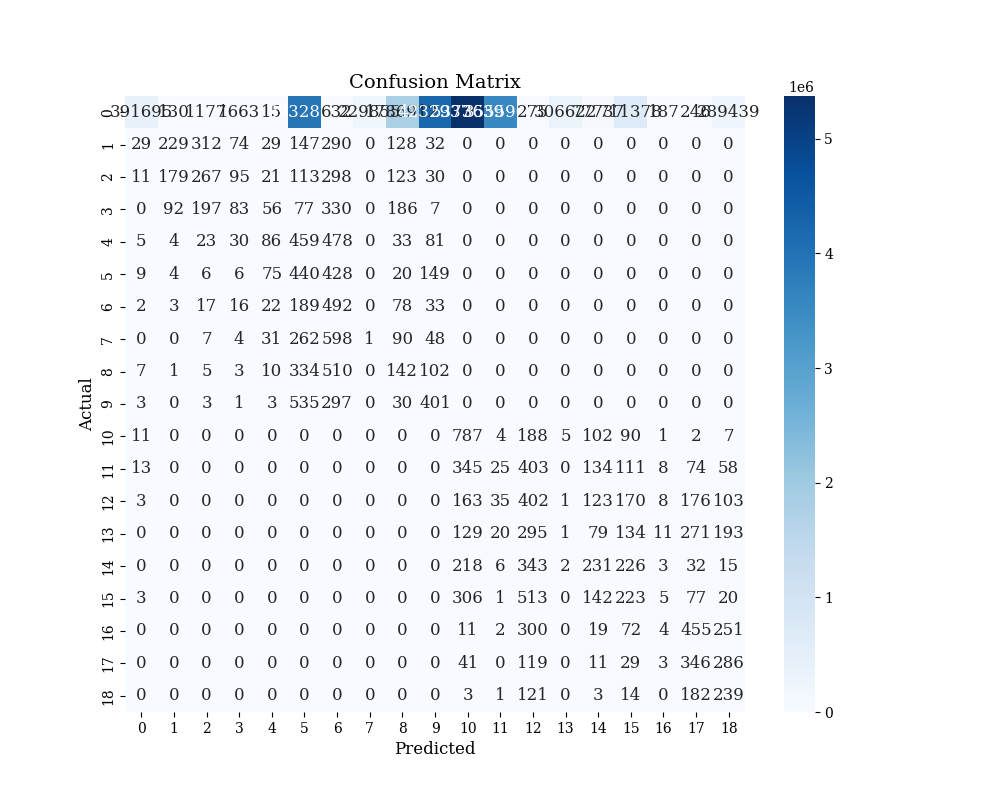
\includegraphics[width=\linewidth]{confusion.png}\\
  {\scriptsize Confusion matrix (top classes).}
\end{column}
\end{columns}
\end{frame}

% ---------------------------------------------------------------------
\begin{frame}{Conclusions \& outlook}
\begin{itemize}
  \item The \textbf{data recipe} (noise-aug difference $+$ NDF negatives $+$ balancing)
        is dominant: $0.08 \to 0.70$.
  \item Mesh-physics GNNs dominate attention GNNs (MeshGraphNet ${\sim}0.76$ vs.\
        published GAT $0.61$); adding front/back cross-ply ``world'' edges
        (\textbf{Hybrid-MGN}) lifts in-distribution to \best{0.792} --- new SOTA,
        just short of $0.80$ (capped by adjacent-layer confusion, not architecture).
  \item \textbf{Size-OOD (unseen 1$\times$1):} detection \emph{generalizes}
        (defect-node recall up to $0.96$) but fine 19-class localization
        \emph{collapses} (defect-only F1 ${\approx}0$) --- a data/representation
        gap, invisible to macro-F1, identical across all architectures.
\end{itemize}
\vspace{0.4em}
\begin{block}{Future work}
  \begin{itemize}
    \item \textbf{Sim-to-real:} transfer to experimental infrared-stress (TSA) data.
    \item \textbf{Physics consistency:} structure-preserving GNNs~\cite{hernandez2022thermodynamics}.
    \item \textbf{Application:} aerospace payload-fairing structural health monitoring.
  \end{itemize}
\end{block}
\end{frame}

% ---------------------------------------------------------------------
\begin{frame}[allowframebreaks]{References}
\printbibliography[heading=none]
\end{frame}

\end{document}
